\documentclass[a4paper]{article}

% font stuff
%\usepackage{mathptmx}
\usepackage{fouriernc}
\usepackage[T1]{fontenc}

\usepackage{amsmath}
\usepackage{amssymb}
\usepackage{amsthm}
\usepackage[retainorgcmds]{IEEEtrantools}
%\usepackage[square]{natbib}

% needs debian package texlive-math-extra
\usepackage{stmaryrd} % for \llbracket, \rrbracket (scott brackets)

\usepackage{tikz}
\usetikzlibrary{positioning}
\usetikzlibrary{matrix}

\newcommand{\arr}{\rightarrow}
\newcommand{\todo}[1]{\bigskip \noindent \emph{todo: #1}}
%\newcommand{\todo}[1]{}
\newcommand{\semantics}[1]{\llbracket #1 \rrbracket}

% They all use the same counter, reset at section boundaries
% This gives a running number:
% Section 1
%   Theorem 1.1
%   Definition 1.2
%   Lemma 1.3
% Section 2
%   Definition 2.1
%   Lemma 2.2
%   ...
\newtheorem{definition}{Definition}[section]
\newtheorem{theorem}[definition]{Theorem}
\newtheorem{lemma}[definition]{Lemma}

\begin{document}

\title{Thesis}
\author{Markus Klinik}
\maketitle

\begin{abstract}

Abstract

\end{abstract}

\section{Introduction}

Introduction

\section{Preliminaries}

  %is a partial order

  %is chain-complete

  %has a least element, i.e.~there is an element $s \in Z$ such that for
    %any other element $t \in Z, s \sqsubseteq t$.

\begin{definition}
A foo is a bar that buzzes.
\end{definition}

\begin{lemma}
Every strict foo frobnicates.
\end{lemma}

\begin{theorem}
\label{thmExample}
The function $p$ is monotone.
\end{theorem}

\begin{proof}
\begin{IEEEeqnarray*}{rCl}
  p(\bot)    & = & \bot   \\
  p(z)       & = & \bot   \\
  p(0)       & = & 0      \\
  p(Sw')     & = & Sp(w') \\
  p(\_w')    & = & p(w')
\end{IEEEeqnarray*}
\end{proof}

As can be seen in \ref{thmExample}, blah blah.

\section{Test}

\begin{definition}
A blub is a snoring blah.
\end{definition}

\begin{lemma}
The world is round.
\end{lemma}


\begin{figure}[ht]
\begin{center}
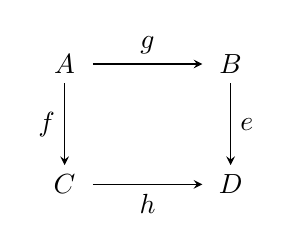
\begin{tikzpicture}
\matrix (m) [matrix of math nodes,row sep=3em,column sep=4em,minimum width=2em]
  {
     A & B \\
     C & D \\
  };
  \path[-stealth]
    (m-1-1) edge node [left] {$f$} (m-2-1)
            edge node [above] {$g$} (m-1-2)
    (m-2-1.east|-m-2-2) edge node [below] {$h$} (m-2-2)
    (m-1-2) edge node [right] {$e$} (m-2-2);
\end{tikzpicture}
\end{center}
\caption{Example of a comutative diagram}
\end{figure}

\begin{figure}
\begin{center}
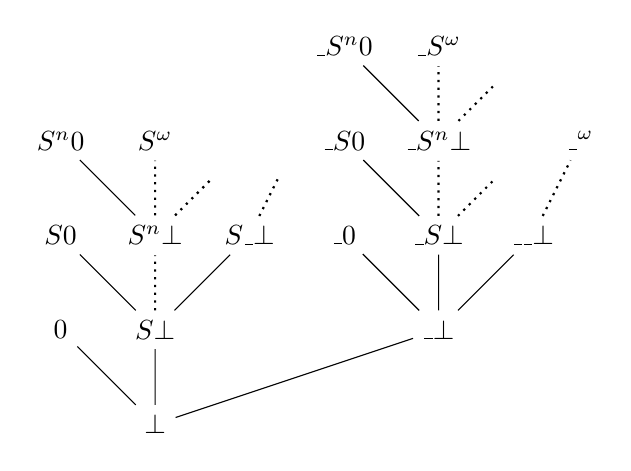
\begin{tikzpicture}
 [ grow'=up
 , scale=1.2
 , level distance=1cm
 , level 1/.style={sibling distance=3cm}
 , level 2/.style={sibling distance=1cm}
 , normal/.style={thin, solid}
 , skipping/.style={thick, dotted}
 , and so on/.style={thick, dotted, sibling distance=0.6cm, level distance=0.6cm}
 ]
  \node {$\bot$}
    child [sibling distance=1cm] { node {$0$} }
    child
    {
      node {$S\bot$}
      child { node {$S0$} }
      child [skipping]
      {
        %node {$SS\bot$}
        %child { node {$SS0$} }
        %child [skipping]
        %{
          node {$S^n\bot$}
          child [normal] { node {$S^n0$} }
          child [skipping] { node {$S^\omega$} }
          child [and so on] {}
        %}
        %child [and so on] {}
      }
      child
      {
        node {$S\_\bot$}
        child [missing] {}
        child [and so on] {}
      }
    }
    child
    {
      node {$\_ \bot$}
      child { node {$\_0$} }
      child
      {
        node {$\_S\bot$}
        child { node {$\_S0$} }
        child [skipping]
        {
          node {$\_S^n\bot$}
          child [normal] { node {$\_S^n0$} }
          child { node {$\_S^\omega$} }
          child [and so on] {}
        }
        child [and so on] {}
      }
      child
      {
        node {$\_\_\bot$}
        child [missing] {}
        %child [missing] {}
        child [skipping] { node {$\_^\omega$} }
      }
    }
  ;
\end{tikzpicture}
\end{center}
\caption{The domain $(Z, \sqsubseteq)$.}
\label{figDomainOfNuF}
\end{figure}

\begin{figure}
\begin{center}
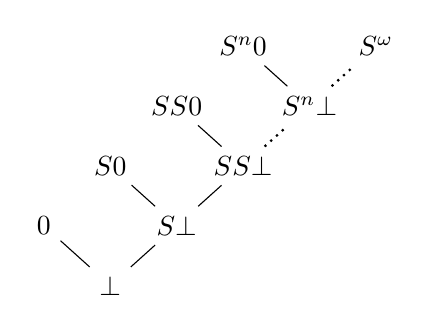
\begin{tikzpicture}[scale=1.2]
  \node {$\bot$} [grow'=up, sibling distance=4.0em, level distance=1.8em]
    child { node {$0$} }
    child
    {
      node {$S\bot$}
      child { node {$S0$} }
      child
      {
        node {$SS\bot$}
        child { node {$SS0$} }
        child [thick, dotted]
        {
          node {$S^n\bot$}
          child [thin, solid] { node {$S^n0$} }
          child { node {$S^\omega$} }
        }
      }
    }
  ;
\end{tikzpicture}
\end{center}
\caption{The domain of $L$, the lazy natural numbers.}
\label{figDomainOfLazyNaturals}
\end{figure}


\section{Further directions}

Left, right, and at the circle stop.

\section{Bibliographic notes}

This work is based on chapter 7 of the PhD thesis of Venanzio Capretta
\cite{Capretta2002}, where coinductive natural numbers are discussed.  Some
treatment of lazy natural numbers can be found in \cite{Escardo1993}.

A short introduction to dentotational semantics can be found in
\cite{Allison1986}, while \cite{Gunter1992} is a more comprehensive treatment of
that topic.  A view on domain theory and denotational semantics from the
perspective of category theory can be found in \cite{Pierce1991},
\cite{Bird1997}, \cite{Mitchell1996} and \cite{BarrWells1990}.


\bibliographystyle{plain}
\bibliography{computer_science}
\end{document}

% vim: textwidth=80
